\documentclass{article}

\usepackage{graphicx}
\usepackage{subfigure}
\usepackage[hypcap]{caption}
\usepackage{listings}
\usepackage{float}
\floatstyle{plaintop}
\restylefloat{table}

\title{Experimental Design and Data Analysis: Assignment 2}
\author{Andrew Bedard(2566978) \& Simone van Gompel(2567525) \\ Group 19}

\begin{document}

  \maketitle

  \section{Exercise 1}
  \subsection*{1}
  Using data from \textit{peruvians.txt} we use the pairs command in R to produce a scatter plot of every variable against every other. The result can be seen in Fig:\ref{fig:Pairs}. From this figure, the variables age and weight seem to have a linear relationship, which would suggest that they are correlated.

    \begin{figure}[!htb]
      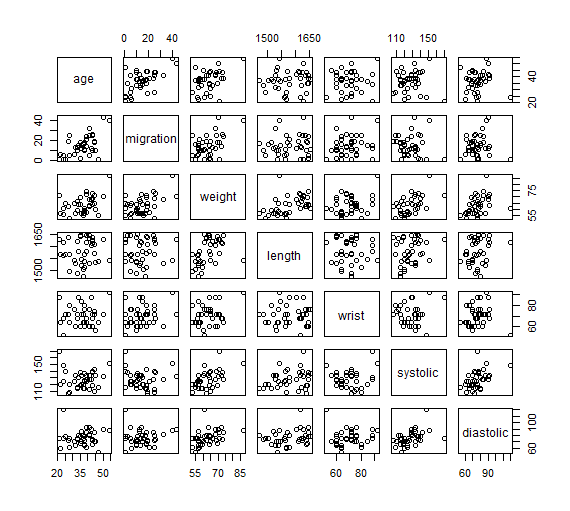
\includegraphics[scale=0.6]{../results/Pairs.png}
      \caption{Pairwise scatterplots of the dataset peruvians}
      \label{fig:Pairs}
    \end{figure}
    
    \subsection*{2}
    Using the Spearman rank correlation test for all variables against migration we obtain the following results:
	\begin{table}
    \begin{center}
    \begin{tabular}{l|llllll}
        \hline 
        & age & weight & length & wrist & systolic & diastolic \\
        \hline
        migration &0.47605753 & 0.35069559 & 0.08458432 & 0.21934983 & -0.16842856 & 0.07514098 \\
        \hline
    \end{tabular}
    \caption{Spearman Rank Correlation test between each variable and \textit{migration} data}
    \label{table:rankcorr}
    \end{center}
    \end{table}
    
    
    The rank correlation between:
    \begin{itemize}
    \item age and migration is 0.47605753, this is visible in Fig\ref{fig:Pairs} in the form of an approximate linear relationship.
    \item weight and migration is 0.35069559, this is visible in Fig\ref{fig:Pairs} as an approximate linear relationship.
    \item Length and migration is 0.08458432, as can be seen in Fig \ref{fig:Pairs}, there is no discernible relationships between the two variables.
    \item wrist and migration is 0.21934983, this result is surprisingly high considering Fig\ref{fig:Pairs}, as any relationship between these two variables is very difficult to see.
    \item systolic and migration is -0.16842856, which is obvious given the very small downward sloping structure seen in Fig\ref{fig:Pairs}.
    \item diastolic and migration is 0.07514098, which is unsurprising considering the lack of structure seen in Fig\ref{fig:Pairs}
    \end{itemize}
    
    \section{Exercise 2}
    \subsection*{1}
    From the data in \textit{clouds.txt}, we can perform various tests to determine whether the two independent samples: values of seeded clouds, and un-seeded clouds are equal.
    \begin{itemize}
    \item The two sample t-test produces:t = 1.9984, df = 33.856, 95\% confidence interval of [-4.7405,559.5859] with mean of x = 441.9846 mean of y = 164.5619 and a p-value of 0.05375, which suggests that we accept the null hypothesis, and thus our samples are the same, this is misleading however. Consider Fig\ref{fig:clouds}, and Fig \ref{fig:normal}; The two sample t-test assumes that both our samples come from a normal population, Fig \ref{fig:normal} represents a randomly generated normally distributed sample of equal size to both seeded and un-seeded cloud data, clearly Fig\ref{fig:clouds} is very different, thus this assumption that our samples are from a normal population is not reasonable, and the two sample t-test is not suitable for this data as is.
    \item The Mann-Whitney test gives: W=473 with a p-value of 0.01383, suggesting that we reject the null hypothesis, and thus, our samples are not equal. The Mann-Whitney test makes no assumptions about the nature of the data but combine our samples to measure their differences, so it is suitable in this case.
    \item The Kolmogorov-Smirnov test gives: D= 0.4231 with a p-value of 0.01905, suggesting that we reject the null hypothesis and that our samples are not equal. The Kolmogorov-Smirnov test measures the differences in the histograms between the two sets of data, and with no constraints on the requirements for our data, this test is suitable.
    \end{itemize}
    
    \begin{figure}[!htb]
      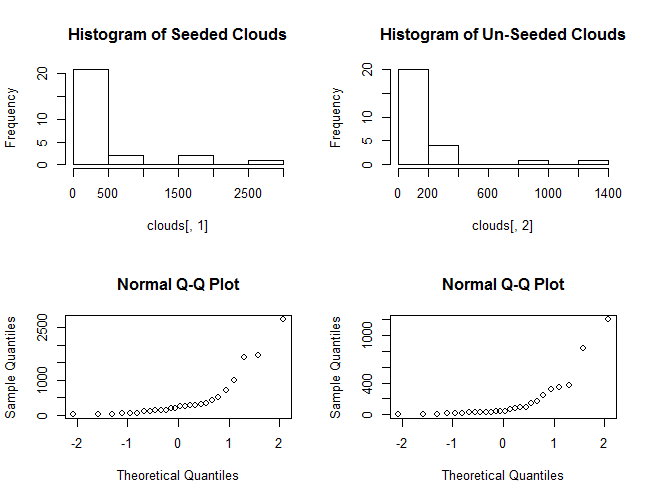
\includegraphics[scale=0.5]{../results/2_1.png}
      \caption{Histograms and QQ-Plots of Seeded Clouds and Un-Seeded Clouds respectively}
      \label{fig:clouds}
    \end{figure}
     
    \subsection*{2}
    We repeat the previous procedure after taking the square root of each data point from both seeded and un-seeded cloud samples.
    \begin{itemize}
    \item The two sample t-test produces t=2.4246, df = 43.363, and a p-value of 0.01956, which suggests that we reject the null hypothesis and that our two samples are not equal. In this case the 95\% confidence interval is [1.2021,13.0713] with mean x=17.068 and mean y= 9.9313. The transformed data, seen in Fig\ref{fig:sq(clouds)} is still too far from normal for the t-test to be suitable in this case.
    \item The Mann-Whitney test gives: W=473 with a p-value of 0.01383, suggesting that we reject the null hypothesis, and thus, our samples are not equal. This is the same result as the original data, which is unsurprising considering the test measures the ranks of a combined sample, once again this test is suitable.
    \item The Kolmogorov-Smirnov test gives: D= 0.4231 with a p-value of 0.01905, suggesting that we reject the null hypothesis and that our samples are not equal. Again, this is the same result obtained with the original data, and as this test only measures the difference between histograms, it is again suitable.
    \end{itemize}
    
    \begin{figure}[!htb]
      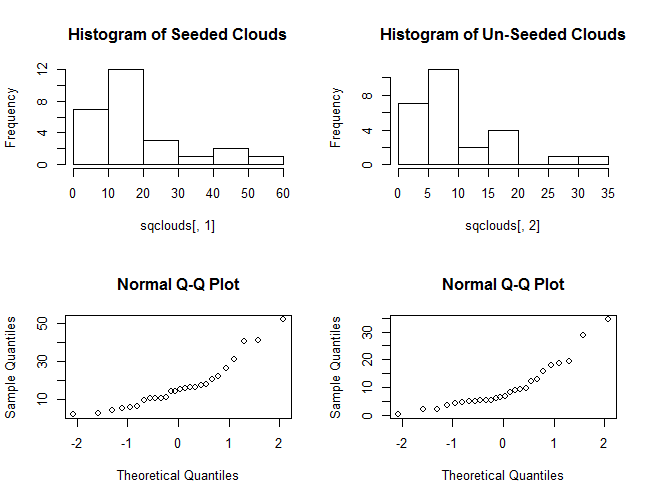
\includegraphics[scale=0.5]{../results/2_2.png}
      \caption{Histograms and QQ-Plots of Seeded Clouds and Un-Seeded Clouds after taking the square root of each data point}
      \label{fig:sq(clouds)}
    \end{figure}
    
    \subsection*{3}
    We repeat the same procedure again, now obtaining the square root of the square root of the original data point in our samples seeded and un-seeded clouds.
    \begin{itemize}
    \item The two sample t-test produces: t=2.5968, df = 48.826, p-value=0.0124, 95\% confidence interval [0.2196,1.7236], mean x = 3.8789 and mean y = 2.9073. This suggests that we reject the null hypothesis, and that our samples are not equal. If we observe Fig\ref{fig:sqsqclouds}, the data is apparently normal, thus this test is suitable in this case.
    \item The Mann-Whitney test gives: W=473 with a p-value of 0.01383, suggesting that we reject the null hypothesis, and thus, our samples are not equal. This is the same result as obtained in both cases before, once again this test is suitable.
    \item The Kolmogorov-Smirnov test gives: D= 0.4231 with a p-value of 0.01905, suggesting that we reject the null hypothesis and that our samples are not equal. Again, this is the same result obtained in the previous two cases, and it is again suitable.
    \end{itemize}
    
    \begin{figure}[!htb]
      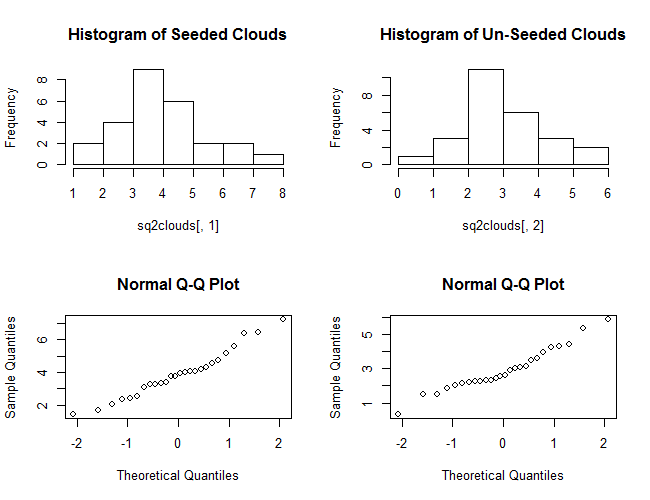
\includegraphics[scale=0.5]{../results/2_3.png}
      \caption{Histograms and QQ-Plots of Seeded Clouds and Un-Seeded Clouds after taking the square root of each data point twice}
      \label{fig:sqsqclouds}
    \end{figure}
    
    \begin{figure}[!htb]
      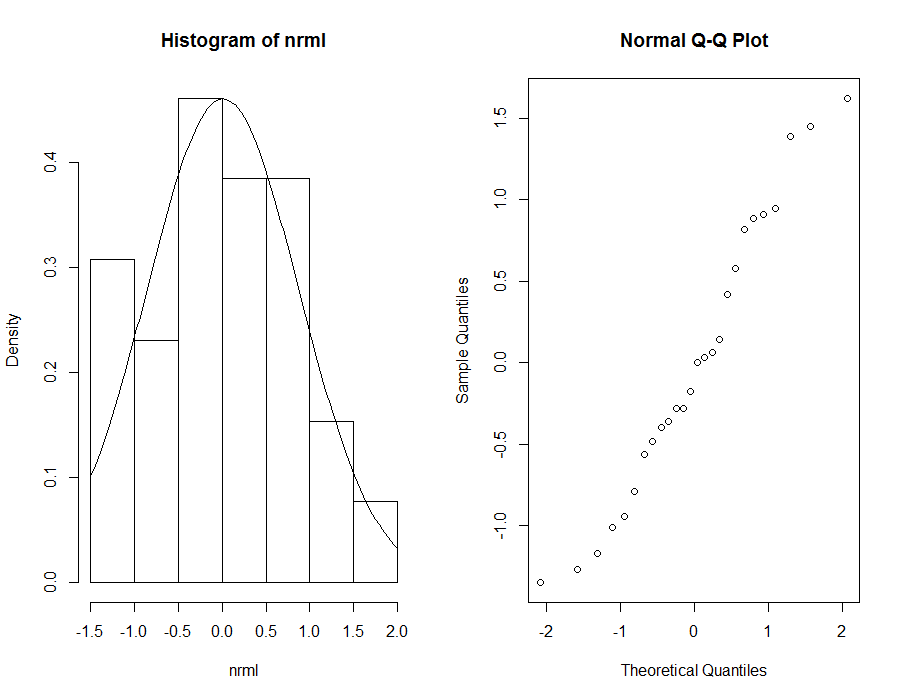
\includegraphics[scale=0.3]{../results/2_3_nrml.png}
      \caption{Histogram and QQ-Plot of randomly generated normally distributed data of same size as both Seeded and Un-Seeded Clouds}
      \label{fig:normal}
    \end{figure}
    
    \section{3}
    \subsection*{1}
    
    \begin{figure}[!htb]
    \centering
      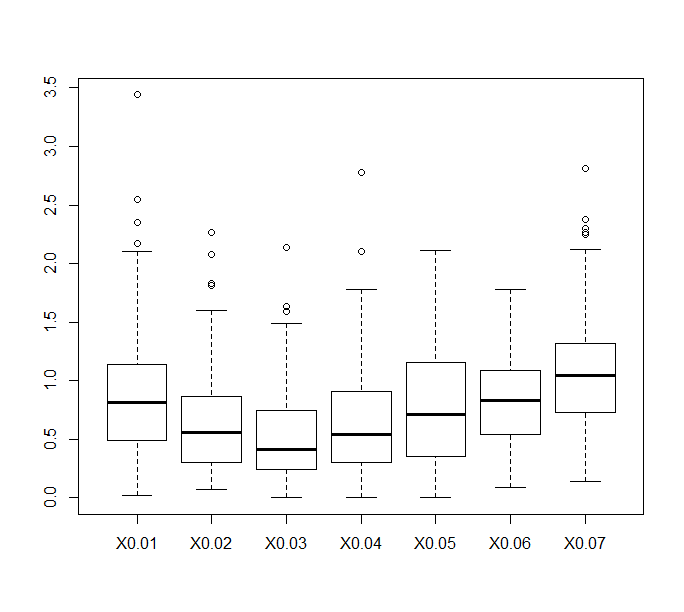
\includegraphics[scale=0.3]{../results/3_1.png}
      \caption{Box Plot of mutation factor and the resulting minimum result obtained}
      \label{fig:box}
    \end{figure}
    
    \subsection*{2}
    
    \begin{figure}[!htb]
      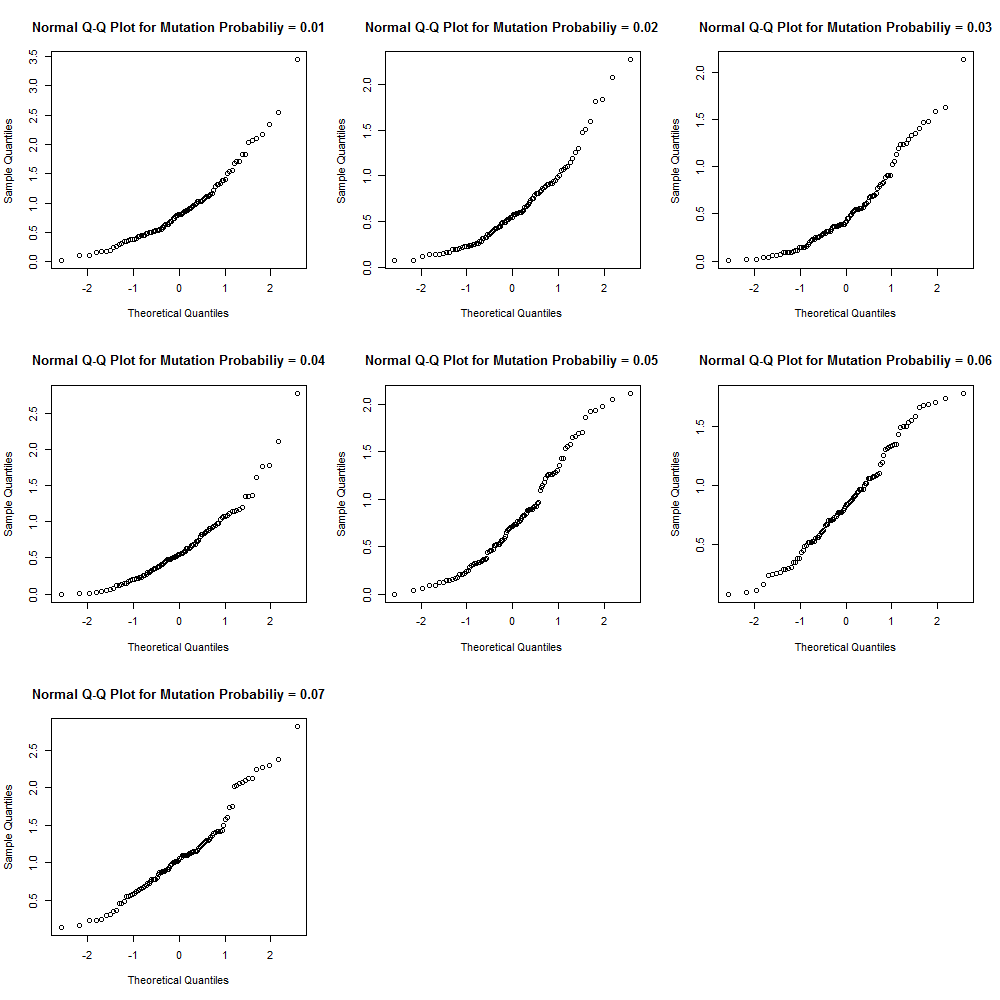
\includegraphics[scale=0.4]{../results/3_2_1.png}
      \caption{QQ-Plots for each mutation factor}
      \label{fig:qq-genal}
    \end{figure}
    
    \begin{figure}[!htb]
    \centering
      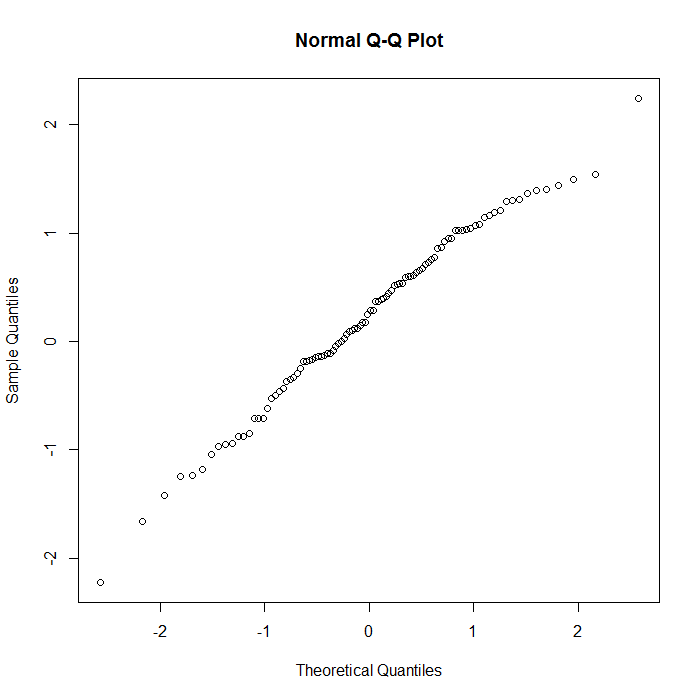
\includegraphics[scale=0.3]{../results/3_2_2.png}
      \caption{QQ-Plot of randomly generated normally distributed population of the same size as those in \textit{genal.txt}}
      \label{fig:qq-nrml}
    \end{figure}
    
    No
    
    \subsection*{3}
    
    \begin{figure}[!htb]
      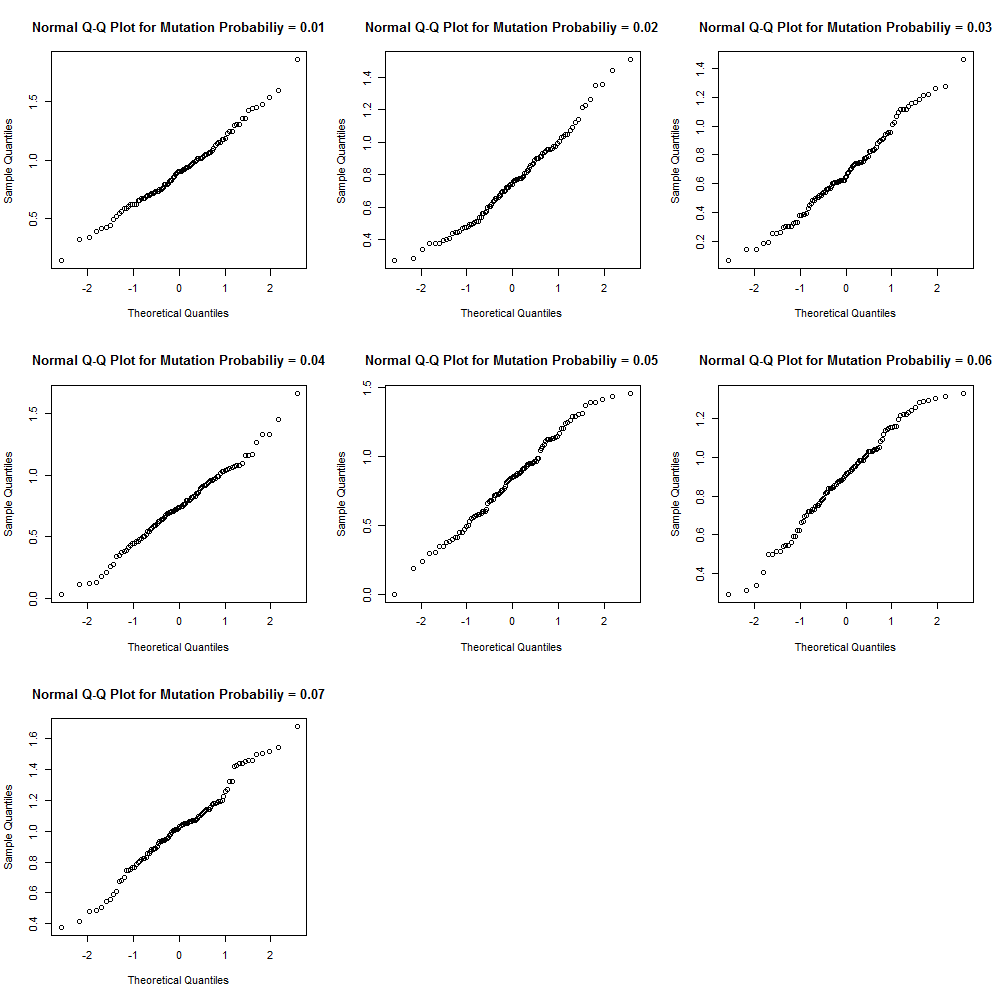
\includegraphics[scale=0.4]{../results/3_3.png}
      \caption{QQ-Plot for each mutation factor after take the square root of each data point}
      \label{fig:qq-sqgenal}
    \end{figure}
    
    Yes
    
    \subsection*{4}
    
    Using sq(genal) we find a p-value of 2.2e-16, therefore we reject the null hypothesis
    
    \subsection*{5}
    
    Based on summary(sqaov) X=0.03 is the best, because 0.9033-0.2227 is the smallest value, and we are estimating the smallest value obtained from an optimization where smaller is better.
    
    \subsection*{6}
    
    \begin{figure}[!htb]
    \centering
      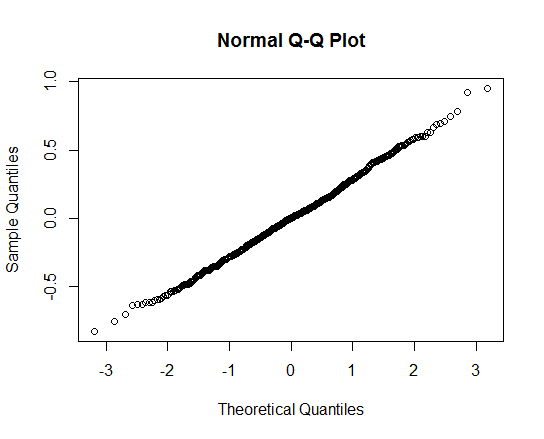
\includegraphics[scale=0.4]{../results/3_6.png}
      \caption{QQ-Plot of the residuals of 1-way Anova test}
      \label{fig:qq-resid}
    \end{figure}
    
    \section{4}
    \subsection*{1}
    
    \begin{figure}[!htb]
    \centering
      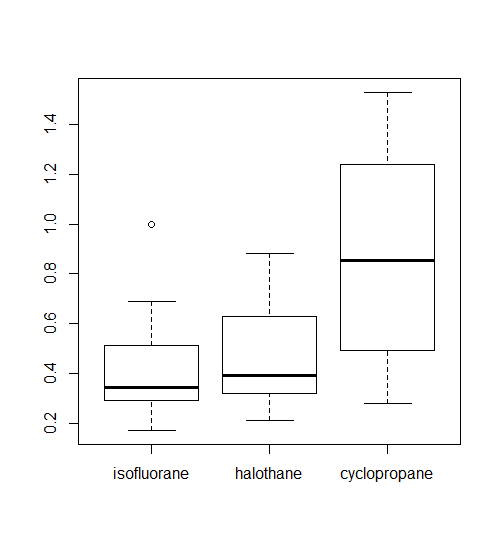
\includegraphics[scale=0.3]{../results/4_1.png}
      \caption{Box plot of plasma epinephrine concentrations under various anaesthesias}
      \label{fig:dbox}
    \end{figure}
    
    \subsection*{2}
    
    \begin{figure}[!htb]
    \centering
      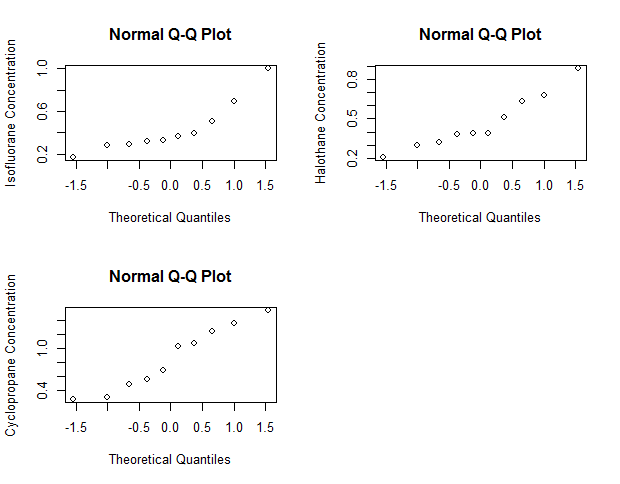
\includegraphics[scale=0.4]{../results/4_2.png}
      \caption{QQ-Plots for data from each type of anaesthesia}
      \label{fig:qq dog}
    \end{figure}
    
    No, the sample sizes are far too small to reasonably judge whether or not they are normal populations.
    \subsection*{3}
    Reject the null, p-value 0.011, estimated value of Isofluorane: 0.4340, of Halothane: 0.469 and of Cyclopropane: 0.853
    \subsection*{4}
    The Kruskal-Wallis test for the same hypothesis gives a p-value of 0.05948, thus we do not reject the null hypothesis. 
    \subsection*{5}
    The differences between the 1-way Anova and the Kruskal-Wallis test could be explained by our initial assumption that the 3 samples represented in the data do not in fact come from a normal population, because 1-way Anova assumes that we are sampling from normal populations this could produce conflicting results, though as we see in Figure \ref{fig:dog-resid} the residuals do not deviate from the normal significantly.
    It is perhaps more compelling that the differences between the 1-way Anova and the Kruskal-Wallis are due to the fact that 1-way Anova assumes our populations have equal population variances, and as is observed in Figure \ref{fig:dbox}, they are obviously not equal.
    
    \begin{figure}[!htb]
    \centering
      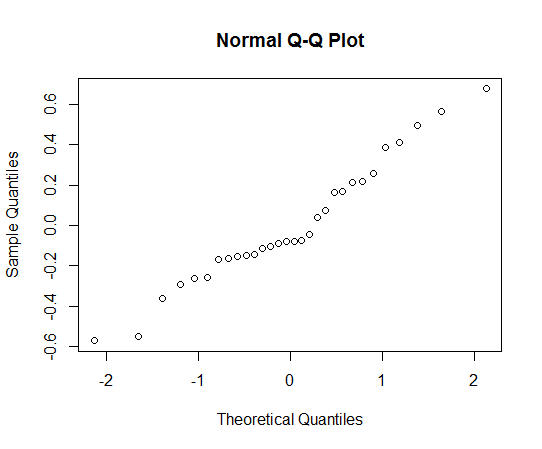
\includegraphics[scale=0.3]{../results/4_5.png}
      \caption{QQ-Plot of residuals of 1-way Anova analysis}
      \label{fig:dog-resid}
    \end{figure}
    
    \section{R-Code}
    \subsection{Exercise 1}\label{sec:RE1}
      \begin{lstlisting}[language=R]
      #1.1
peru = read.table("peruvians.txt", header=T)
peru = peru[,-c(5,6,7)]
pairs(peru)

#1.2
#This shows the spearman rank correlation against all variables
correl_s = cor(peru, method="spearman")

correl_s[2, ]
      \end{lstlisting}
    \subsection{Exercise 2}\label{sec:RE2}
      \begin{lstlisting}[language=R]
      #2.1
clouds = read.table("clouds.txt", header=T)
len = length(clouds[,1])
nrml = rnorm(len)

#Histograms,boxplots,qqplots to see if data is normal
par(mfrow=c(2,2))
hist(clouds[,1])
hist(clouds[,2])
qqnorm(clouds[,1])
qqnorm(clouds[,2])
#These graphs should show the data is not normal

#Two sample t-test 
t.test(clouds[ ,1],clouds[ ,2])
#Mann-Whitney test
wilcox.test(clouds[ ,1],clouds[ ,2])
#Kolmogorov-Smirnov test
ks.test(clouds[,1],clouds[,2])

#2.2
sqclouds = sqrt(clouds)

#Histograms,boxplots,qqplots to see if data is normal
par(mfrow=c(2,2))
hist(sqclouds[,1])
hist(sqclouds[,2])
qqnorm(sqclouds[,1])
qqnorm(sqclouds[,2])
#These graphs should show the data is not normal

#Two sample t-test 
t.test(sqclouds[ ,1],sqclouds[ ,2])
#Mann-Whitney test
wilcox.test(sqclouds[ ,1],sqclouds[ ,2])
#Kolmogorov-Smirnov test
ks.test(sqclouds[,1],sqclouds[,2])

#2.3
sq2clouds = sqrt(sqclouds)

#Histograms,boxplots,qqplots to see if data is normal
par(mfrow=c(2,2))
hist(sq2clouds[,1])
hist(sq2clouds[,2])
qqnorm(sq2clouds[,1])
qqnorm(sq2clouds[,2])
#These graphs should show the data is not normal

#Two sample t-test
t.test(sq2clouds[ ,1],sq2clouds[ ,2])
#Mann-Whitney test
wilcox.test(sq2clouds[ ,1],sq2clouds[ ,2])
#Kolmogorov-Smirnov test
ks.test(sq2clouds[,1],sq2clouds[,2])

par(mfrow=c(1,2))
hist(nrml, prob=TRUE)
curve(dnorm(x,mean=mean(nrml),sd=sd(nrml)), add=TRUE)
qqnorm(nrml)
      \end{lstlisting}
    \subsection{Exercise 3}\label{sec:RE3}
      \begin{lstlisting}[language=R]
#3.1
genal = read.table("genal.txt", header=T)
len=length(genal[,1])
nrml=rnorm(len)

par(mfrow=c(1,1));boxplot(genal)

#3.2
#Loops through, creating QQ-plot for each mutation probability
par(mfrow=c(3,3))
for (i in 1:7) {
  qqnorm(genal[,i],
         main =paste("Normal Q-Q Plot for Mutation Probabiliy =",
                     i/100))
}
#qqplot of normal random sample of same size as genal[,i]
par(mfrow=c(1,1));qqnorm(nrml)
#3.3
sqgenal=sqrt(genal)

#Loops through, creating QQ-plot for each mutation probability
par(mfrow=c(3,3))
for (i in 1:7) {
  qqnorm(sqgenal[,i],
         main =paste("Normal Q-Q Plot for Mutation Probabiliy =",
                     i/10))
}

#3.4

#Create data-frames for the origional genal data, 
#and the squareroot genal data
sqframe=data.frame(yield=as.vector(as.matrix(sqgenal)),
                      variety=factor(rep(1:7,each=100)))

sqaov=lm(yield~variety,data=sqframe)
anova(sqaov)

#3.5
summary(sqaov)

#3.6
par(mfrow=c(1,1));qqnorm(residuals(sqaov))

      \end{lstlisting}
    \subsection{Exercise 4}\label{sec:RE4}
      \begin{lstlisting}[language=R]
      #4.1

dogs = read.table("dogs.txt", header=T)
len=length(dogs[,1])
boxplot(dogs)

#4.2
par(mfrow=c(2,2))
qqnorm(dogs[,1],ylab="Isofluorane Concentration")
qqnorm(dogs[,2],ylab="Halothane Concentration")
qqnorm(dogs[,3],ylab="Cyclopropane Concentration")

#4.3
dogframe = data.frame(yield=as.vector(as.matrix(dogs)),
                      variety=factor(rep(1:3,each=10)))
dogaov=lm(yield~variety,data=dogframe)
anova(dogaov)
summary(dogaov)

#Calculate expected value
u1=0.4340; 
u2=0.0350+u1
u3=0.4190+u1

print(u1,u2,u3)
#4.4

attach(dogframe)
kruskal.test(yield,variety)
par(mfrow=c(1,1));qqnorm(dogaov$residuals)

#Calculate and print population variances
for (i in 1:3){
  print(sum((dogs[,i]-mean(dogs[,i]))^2)/(len-1))
}
      \end{lstlisting}
\end{document}
